\section{Сеть Asure}

Сеть Asure состоит из клиентов узлов, в которых блокчейн Asure работает и синхронизируется между отдельными узлами с помощью консенсуса. Для достижения количества требуемых транзакций нагрузка должна быть распределена по нескольким цепочкам блоков. Одна или несколько цепочек блоков могут быть специфичны для одной системы социального обеспечения.  Чтобы извлечь выгоду из экосистемы, большая добавленная стоимость для масштабируемости возникает только тогда, когда активы могут быть переданы между несколькими блокчейнами. Кроме того, специализированные сайдчейны могут извлечь выгоду из безопасности рутчейна и таким образом, активы будут лучше защищены. \cite{omisego}

\subsection{Требования}
Основные требования к социальному обеспечению и блокчейну в масштабируемом сценарии:

\subsubsection*{Пропускная способность транзакций}
Сеть Asure должна быть способна масштабировать пропускную способность транзакций через сайдчейны до такой степени, чтобы страны и резиденты могли совершать свои финансовые транзакции в пределах внешней цепи.

\subsubsection*{Конфиденциальность}
Чтобы защитить конфиденциальность пользователей, никакие личные данные не могут храниться в блокчейне. По возможности, транзакции не должны назначаться пользователю. Персональные данные зашифрованы и хранятся вне блокчейна. Используя метод Zero-Knowledge-Proof (Доказательство с нулевым разглашением), можно полностью избежать хранения личных данных. 

Для того чтобы социальное обеспечение на основе блокчейна было установлено, оно должно соответствовать руководящим принципам защиты данных и конфиденциальности национальных и международных норм, таких как Общее положение о защите данных (GDPR) в Европейском союзе. \cite{gdpr}

\subsubsection*{Прозрачность}
Прозрачность в сети Asure является важным фактором защиты систем социального обеспечения от коррупции и манипуляций. Уважая конфиденциальность пользователей, важно обеспечить прозрачность системы, в целом, чтобы включить например статистику общего денежного потока в реальном времени.

\subsubsection*{Бизнес-правила для системы}
Социальное обеспечение имеет много влияющих факторов и правил, которые должны выполняться, адаптироваться и осуществляться, поэтому мы обязаны иметь возможность выполнять собственные бизнес-правила в сайдчейне с EVM или EWASM.

\subsubsection*{Безопасность}
Система, которая организует и хранит финансовые транзакции систем социального обеспечения, должна удовлетворять множественным требованиям безопасности. Необходимо убедиться, что данные не могут быть обработаны или украдены, а система устойчива к атакам, сбоям и другим ошибкам.

\subsection{Другие технологии}
Пун и Бутерин представили платформу Plasma в 2017 году для решения проблемы масштабирования путем организации нескольких независимых блокчейнов в древовидную иерархию. Последовательные предложения Plasma описали места вне цепи для простых передач взаимозаменяемых и не взаимозаменяемых токенов. Эти предложения включают Plasma MVP, Plasma Cash и Plasma Debit. Платформа Plasma находится в стадии активного исследования и в зависимости от применения и требований, реализация Plasma варьируется.\cite{plasma} Loom и OmiseGO являются одними из первых, кто внедряет платформу Plasma и продолжает свои исследования в этой области. 

Платформа Plasma была представлена совсем недавно и является одним из наиболее многообещающих предлагаемых решений для масштабируемых вычислений на блокчейн. Plasma имеет очень обширную белую книгу, но не содержит всей технической информации, необходимой для немедленной реализации. Plasma может обеспечить масштабируемость для приложений на Ethereum. Это специфический для приложения протокол сайдчейна.

С другой стороны, Polkadot был представлен Gavin Wood (Гэвином Вудом) в 2017 году. Целью концепции является создание гетерогенного многоцепного решения, которое позволяет соединять индивидуально адаптированные сайдчейны с общедоступными блокчейнами. Polkadot позволяет различным блокчейнам обмениваться сообщениями безопасным и надежным способом.

Raiden Network это решение для автономного масштабирования с технологией платежей и каналов связи, позволяющее осуществлять почти мгновенные и с низкой комиссией, масштабируемые платежи. Он дополняет блокчейн Ethereum и работает с любым токеном, совместимым с ERC20.

\subsection{Plasma}
Сеть Asure будет использовать платформу Plasma для создания масштабируемой сети блокчейнов для реализации потребностей систем социального обеспечения. 

Чтобы еще больше повысить ограничения уровня 1 для эффективного функционирования системы социального обеспечения, масштабирование уровня 2 считается наиболее эффективным решением. Это облегчает реализацию безопасности в системе, поскольку она опирается на уровень 1. Решение будет спроектировано как комбинация рутчейна Asure и соответствующего сайдчейна для соответствия всем потребностям систем социального обеспечения.

Сайдчейны Asure могу быть связаны со смарт контрактами Ethereum или любыми другими технологиями блокчейна, которые работают с шаблонами проектирования Plasma.


\begin{figure}[H]
    \centering
    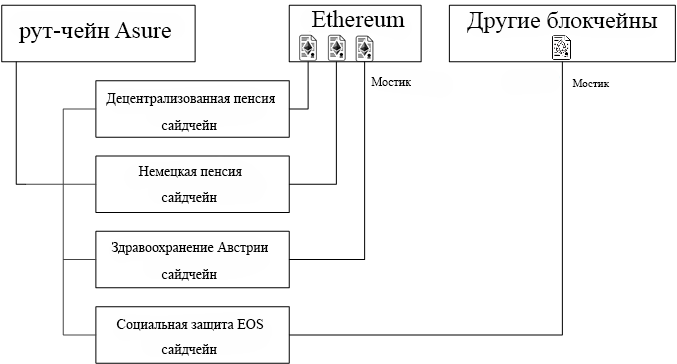
\includegraphics[width=4.0in]{img/chains.png}
    \caption{Сайдчейны Asure}
    \label{fig:asure_side_chains}
\end{figure}
